\documentclass[sigconf]{acmart}
\setcopyright{none}
\settopmatter{printacmref=false}
\acmConference[Kaggle Competition]{Filament Segmentation Challenge}{2026}{\href{https://www.kaggle.com/competitions/filament-segmentation-2026}{kaggle.com/competitions/filament-segmentation-2026}}
\acmBooktitle{Competition Report}
\acmDOI{}
\acmISBN{}

\usepackage{xcolor}
\newif\ifguideStyle
\guideStyletrue
\newcommand{\guide}[1]{%
  \ifguideStyle
    {\color{gray!65}\itshape #1}%
  \fi
}
\usepackage{mathtools}
\usepackage{subcaption}
\usepackage{tabularx}
\usepackage{multirow}

\guideStylefalse

\begin{document}

\title[Structural Proposal Selection for Solar Filaments]{Structural Proposal Selection with Semantic-Guided Refinement for Solar Filament Instance Segmentation}
\subtitle{A Solution to the Solar Filament Segmentation Challenge 2026}
\author{Zhuoer Wang}
\affiliation{%
  \institution{Sichuan University}
  \city{Chengdu}
  \country{China}
}
\email{2025141010321@stu.scu.edu.cn}

\begin{abstract}
This report describes our solution to the Solar Filament Segmentation Challenge~2026, a Kaggle competition on automatic segmentation of solar filaments in GONG H-$\alpha$ observations. The solution combines four-view instance proposals, semantic-probability-guided contour correction, relational quality prediction, and risk-aware instance selection. The semantic ensemble supplies pixel-level evidence, while the instance proposals preserve alternative object identities. The final configuration, Fusion H6a, obtained historical development and audit panoptic quality (PQ) of 0.465532 and 0.475113, respectively. Its public leaderboard score displays 0.40. The archived submission contains 1,268 disjoint instance masks. Source and replay instructions are available in the \href{https://github.com/wangzgui/solar-filament-segmentation-2026}{public GitHub repository}.
\end{abstract}

\maketitle

\section{Introduction}
This report goes over the details of our submitted solution to the Solar Filament Segmentation Challenge~2026 \cite{filament-segmentation-2026}. The challenge, launched on July~10,~2026, is organized by the Earth-Space AI Research (ESAIR) Lab\footnote{\href{https://www.esairlab.com/home}{www.esairlab.com/}}. This challenge utilizes the MAGFiLO dataset for evaluation of the segmentation algorithms \cite{ahmadzadeh2024dataset}.

Thin extensions and adjacent filaments make the boundaries of individual masks difficult to assign. A detector can preserve object identity while missing a faint extension. A dense foreground map can recover that extension while also connecting unrelated objects. We use the dense probabilities to correct local contours and the candidate set to decide which objects to output. Figure~\ref{fig:pipeline} shows the sequence used for the final submission.

\section{Methodology}\label{sec:methodology}

\subsection{Instance models and training}
The instance stream starts from a Mask R-CNN detector \cite{he2017mask} and instance-conditioned U-Net refiner \cite{ronneberger2015unet}. Preprocessing estimates disc geometry and corrects radial brightness before inference. The A1 adaptation uses a ResNet-50 feature pyramid \cite{lin2017fpn} at 1536-pixel detector resolution. Starting from the V1 detector, SGD runs for four epochs with initial learning rate 0.001. The adaptation uses 343 fitting and 85 tuning photos and the signed inference checkpoint is from epoch three. The frozen V1 refiner uses a ResNet-18 U-Net with 384-pixel crops and five channels: three grayscale copies, continuous coarse-mask probability, and radial position. V1 trains this model for eight epochs with AdamW, cosine decay, and equal BCE and Tversky loss weights. The repository contains the original V1 and A1 training workflows.

Mul2 runs two flips and two quarter-turns and aligns all masks to the native $2048\times2048$ grid. A conservative vote result yields reference instances $A$. Alternatives $D$ come from the four aligned donor streams. We deduplicate equal masks, retain provenance and scores, and discard donors below 96 pixels. View agreement strengthens the evidence for a reference identity. Disagreement preserves plausible alternatives for later selection.

\begin{figure}[t]
  \centering
  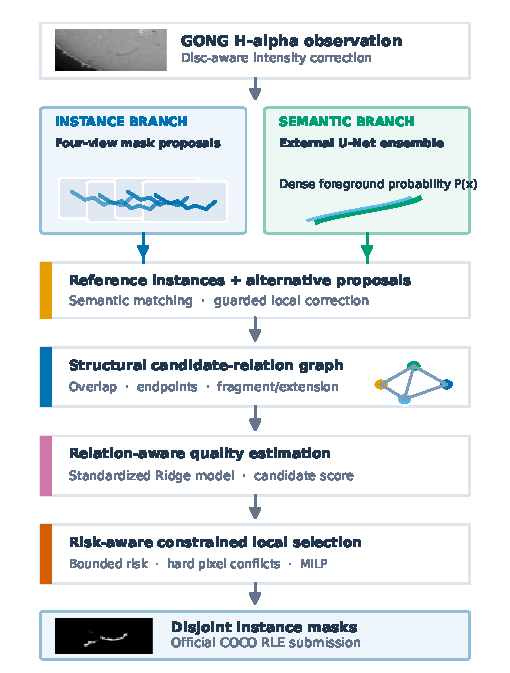
\includegraphics[width=.87\columnwidth]{pipeline.pdf}
  \caption{Inference flow. Multi-view instance masks and the independent foreground ensemble meet at local contour correction and candidate scoring. The final constrained decision produces disjoint instances.}
  \Description{Flowchart from disc-normalized GONG imagery through separate instance and semantic branches, joined by contour correction, quality estimation, and constrained selection.}
  \label{fig:pipeline}
\end{figure}

\subsection{Dense semantic evidence and contour correction}
Afshar's public ensemble \cite{afshar2026solar} provides a foreground probability map $P(x)$ on the native grid. We use five ResNet-34 and five EfficientNetV2-S U-Nets and average eight dihedral views. In the historical evaluation, the matched semantic predictions use the corresponding fold assignments. The signed ten-model ensemble predicts the test images.

For a reference mask $M$ and its matched semantic component $U$, F4 considers edits within exterior and interior three-pixel bands $B_3^+(M)$ and $B_3^-(M)$:
\begin{align*}
A^+ &= (U\setminus M)\cap B_3^+(M)\cap\{P\geq0.55\},\\
A^- &= (M\setminus U)\cap B_3^-(M)\cap\{P\leq0.22\}.
\end{align*}
The contour rule protects the common core, restricts propagation to eight-connected pixels, enforces pixel ownership, and rejects edits that change the instance's component count. This keeps a connected semantic component from absorbing the identities of adjacent instances. The final selection step uses these corrected contours and the original donor masks.

\subsection{Relational quality estimation}
The candidate graph has nodes $C=A\cup D$. Node descriptors include detector confidence, area, elongation, radial position, view agreement, component count, and three semantic summaries (mean probability, high-probability fraction, and boundary contrast). Pairwise overlap, containment, skeleton endpoints, and principal-axis alignment identify duplicates, potential fragments, extensions, and nearby competition. The neighborhood radius is 36 pixels, and endpoint-based extension evidence requires alignment of at least 0.80.

For candidate $c_i$, annotation views $V$ and view-specific mask sets $G_v$, the training target is
\[
y_i=\frac{1}{|V|}\sum_{v\in V}\max_{g\in G_v}
\left[\operatorname{IoU}(c_i,g)\mathbf{1}\{\operatorname{IoU}(c_i,g)>0.5\}\right].
\]
An empty ground-truth set contributes zero. A standardized Ridge model ($\alpha=12$) uses these view-averaged targets and per-photo weighting. The development cohort uses leave-one-date-out predictions. The refit uses development labels for scoring the historical audit cohort and Test. Audit labels are reserved for evaluation.

\subsection{Risk-aware set selection}
The selection unit is a local candidate set. Let $q_i$ denote estimated quality and $\lambda$ the archived decision price. H6a applies a small bounded downward adjustment to contested or weak reference candidates:
\[
\widetilde q_i=q_i-0.035\,\operatorname{clip}\bigl((\lambda+0.02-q_i)/0.16,0,1\bigr).
\]
The weakness tests use view support, semantic support, fragment evidence and competition. Each eligible candidate has a utility $u_i=\widetilde q_i-\lambda-\eta_i$ after policy costs. Let $E_h$ be hard pixel conflicts and $E_s$ soft fragment relations. The objective and primary conflict constraint are
\begin{align*}
\max_{z\in\{0,1\}^{|C|}}\;&\sum_i u_i z_i-\sum_{(i,j)\in E_s}\rho_{ij}z_i z_j,\\
&z_i+z_j\leq1,\quad (i,j)\in E_h.
\end{align*}
Local mixed-integer solves also enforce reference protections and conditional donor eligibility. The frozen H6a policy returns a subset of available masks. Every final instance is checked for nonzero area and disjoint pixel ownership, then encoded as COCO RLE. Figure~\ref{fig:examples} shows two predictions decoded from the submitted CSV.

\begin{figure*}[t]
  \centering
  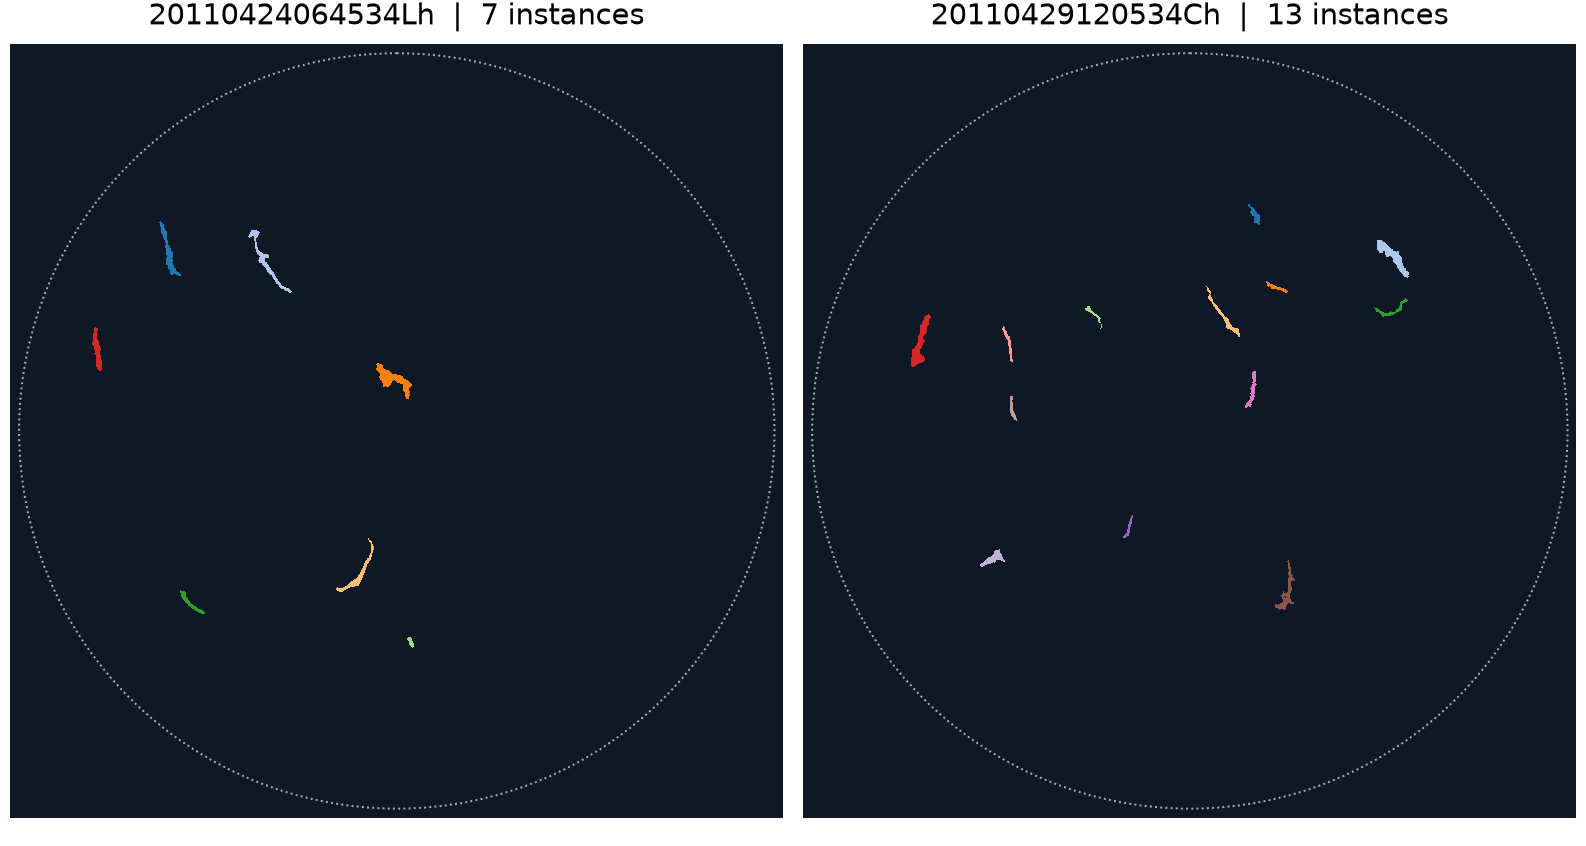
\includegraphics[width=.88\textwidth]{segmentation_examples.png}
  \caption{Two native-grid test predictions from the signed Fusion H6a CSV. Colors distinguish instance identities within each panel. The dotted disc is an orientation guide for the full mask canvas.}
  \Description{Two full-disc instance mask canvases, one showing seven predicted filaments and the other showing thirteen.}
  \label{fig:examples}
\end{figure*}

\section{Evaluation}\label{sec:evaluation}
\subsection{Protocol}
With one-to-one IoU matches strictly above 0.5, the official scoring implementation pools across annotation views:
\[
\mathrm{PQ}=\frac{\sum_{\text{matched}}\mathrm{IoU}}
{\mathrm{TP}+(\mathrm{FP}+\mathrm{FN})/2}.
\]
We distinguish the 140-photo historical V1 ablation, the later 16-photo development and 19-photo audit cohorts, and public leaderboard results. Development and audit use fixed date-separated roles. Both are repeatedly inspected historical cohorts with possible upstream training exposure. These data support paired retrospective comparisons. They offer limited evidence about generalization to new dates and sites.

\subsection{Detector and refiner}
We compare detector output and detector plus refiner under the same default policy on 140 historical V1 photos (204 annotation views). Table~\ref{tab:v1} shows a PQ gain of 0.01266, with 26 more matched instances across annotation views, one fewer FP, and 26 fewer FN. The same archive reports 0.39274 PQ in a separate detector-confidence calibration trial at 0.70. The detector-plus-refiner row uses the default 0.50 operating point.

\begin{table}[h]
\caption{Paired historic V1 model-stage comparison.}
\label{tab:v1}
\centering
\begin{tabular}{@{}lrrrr@{}}
\toprule
Stage & PQ & TP & FP & FN \\
\midrule
Detector & .35928 & 915 & 939 & 509 \\
Detector + refiner & .37194 & 941 & 938 & 483 \\
\bottomrule
\end{tabular}
\end{table}

\subsection{Integrated system and semantic complementarity}
On the later paired cohorts, the final system raises PQ by 0.01462 on development and 0.01340 on audit compared with the multi-view reference (Table~\ref{tab:later}). The semantic contour correction contributes a large share of the development gain. On the 19-photo audit cohort, the independently scored semantic ensemble matches 22 ground-truth instances across views missed by the multi-view result, and the multi-view result uniquely matches 21. Both match 141 and neither matches 62. These coverage counts describe complementary evidence and do not measure the gain available under final instance-set constraints.

\begin{table}[h]
\caption{Cumulative comparisons on the later paired cohorts.}
\label{tab:later}
\centering
\begin{tabular}{@{}lrr@{}}
\toprule
System & Dev.\ PQ & Audit PQ \\
\midrule
Mul2 multi-view reference & .45091 & .46171 \\
F4 semantic contour correction & .46313 & .46343 \\
C1b relation-aware filtering & .46540 & .47029 \\
C5 joint candidate selection & .46223 & .47313 \\
Fusion H6a submitted policy & .46553 & .47511 \\
\bottomrule
\end{tabular}
\end{table}

H6a exceeds C5 by 0.00330 PQ on development and 0.00198 on audit, mainly through FP reduction. Both submissions display 0.40 on the public leaderboard, where H6a ranked higher. The unrounded difference is unavailable. The exact H6a file contains 1,268 disjoint masks on 179 of the 180 test photos and is identified by the SHA-256 prefix \texttt{0d170beedd870d53}. The repository records the complete digest, configuration, and cohort-level results. The final-stage cached replay and the much more expensive upstream network execution are described separately in its reproduction guide.

\subsection{Failure cases and remaining work}
The H6a audit retained 167 matched annotation-view instances, alongside 65 FP and 79 FN. Among the matches, 33 have IoU between 0.5 and 0.6. Faint terminal branches, fragmented masks and neighboring objects that appear connected remain important sources of error. A dense foreground map helps recover contour detail, while choosing whether a competing mask should be an independent instance depends on its relationship to its neighbors.

We also evaluated explicit graph-based reconstruction using hierarchical foreground components and skeleton paths. A low-cost bridge can join two distinct filaments, while a split can damage a correct instance. The final submission uses graph-derived features for scoring and conflict decisions. An exploratory joint structural branch improved audit PQ by 0.01251, fell by 0.00690 on development, and displayed 0.39 when submitted. This is consistent with a small number of historical fixes failing to transfer across the images modified at test time.

Follow-up work should test improved proposal recall and instance-conditioned shape refinement on dates and observatories held out from upstream training. Independent annotation views would help distinguish repeatable boundary failures from annotator disagreement. Reporting required checkpoints, split membership and the signed output makes the effect of an individual pipeline stage easier to verify.

\section{Acknowledgment}\label{sec:acknowledgment}
The organization of the Filament Segmentation Challenge 2026 is partially supported by the U.S. National Science Foundation (NSF) under Grant No. 2209912 and 2433781, directorate for Computer and Information Science and Engineering (CSE), and Office of Advanced Cyberinfrastructure (OAC), and Grant No. 2511630, AST Division Of Astronomical Sciences and MPS Directorate for Mathematical and Physical Sciences.

The Filament Segmentation Challenge 2026 is sponsored by the U.S. National Science Foundation (NSF) National Solar Observatory (NSO).

This work utilizes GONG data obtained by the NSO Integrated Synoptic Program, managed by the National Solar Observatory, which is operated by the Association of Universities for Research in Astronomy (AURA), Inc. under a cooperative agreement with the National Science Foundation and with contribution from the National Oceanic and Atmospheric Administration. The GONG network of instruments is hosted by the Big Bear Solar Observatory, High Altitude Observatory, Learmonth Solar Observatory, Udaipur Solar Observatory, Instituto de Astrofísica de Canarias, and Cerro Tololo Interamerican Observatory.

\bibliographystyle{ACM-Reference-Format}
\bibliography{main}

\end{document}
